\begin{frame}[fragile]
\frametitle{Implementation: Extending the FreeRTOS API}
FreeRTOS MPU creates restricted tasks via \texttt{xTaskCreateRestricted}.
We extend the task creation API with a domain parameter.

\vspace{0.2cm}
\begin{lstlisting}[language=C, basicstyle=\scriptsize\ttfamily]
typedef struct xDOMAIN_PARAMETERS {
  uint32_t ulSliceIndex;   // Start time slice
  uint32_t ulSliceLength;  // Number of slices
} DomainParameters_t;
\end{lstlisting}

\begin{itemize}
  \item When creating a restricted task, one must pass the start of the group of time
slices and their length
\item If no \texttt{DomainParamters\_t} is passed, then it creates the tasks within the current domain
\end{itemize}

\end{frame}

\begin{frame}[fragile]
\frametitle{Implementation: Constant-Time Domain Creation}

\begin{columns}
\begin{column}{0.45\textwidth}
\begin{center}
\small Single domain\\[0.2cm]
\resizebox{\textwidth}{!}{\input{figures/example_timeline_a.tex}}
\end{center}
\end{column}
\begin{column}{0.45\textwidth}
\begin{center}
\small Fragmented domain\\[0.2cm]
\resizebox{\textwidth}{!}{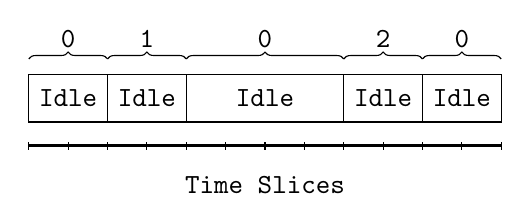
\begin{tikzpicture}[font=\ttfamily]
    % Style for general text nodes
    \tikzset{lbl/.style={inner sep=1pt, align=center}}

    % Define vertical coordinates for rows and labels
    \def\barheight{0.6} % Height of each bar
    \def\vtopprio{1.5}   % Vertical center of the top bar row
    \def\ytimeline{\vtopprio - \barheight} % Vertical position of the minor frames timeline

    % Define standard tick positions
    \def\timeslice{0.5}

    \def\astart{0}
    \def\aend{2}
    \path[draw, decorate, decoration=brace] (\astart, \vtopprio + 0.5) -- (\timeslice * \aend, \vtopprio + 0.5) node[lbl, midway, above, yshift=0.3em]{0};
    \draw (\astart, \vtopprio-\barheight/2) rectangle (\timeslice*\aend, \vtopprio+\barheight/2) 
      node[lbl, midway]{Idle};

    \def\bend{4}
    \path[draw, decorate, decoration=brace] (\timeslice * \aend, \vtopprio + 0.5) -- (\timeslice * \bend, \vtopprio + 0.5) node[lbl, midway, above, yshift=0.3em]{1};
    \draw (\timeslice * \aend, \vtopprio-\barheight/2) rectangle (\timeslice*\bend, \vtopprio+\barheight/2) 
      node[lbl, midway]{Idle};

    \def\cend{8}
    \path[draw, decorate, decoration=brace] (\timeslice * \bend, \vtopprio + 0.5) -- (\timeslice * \cend, \vtopprio + 0.5) node[lbl, midway, above, yshift=0.3em]{0};
    \draw (\timeslice * \bend, \vtopprio-\barheight/2) rectangle (\timeslice*\cend, \vtopprio+\barheight/2) 
      node[lbl, midway]{Idle};

    \def\dend{10}
    \path[draw, decorate, decoration=brace] (\timeslice * \cend, \vtopprio + 0.5) -- (\timeslice * \dend, \vtopprio + 0.5) node[lbl, midway, above, yshift=0.3em]{2};
    \draw (\timeslice * \cend, \vtopprio-\barheight/2) rectangle (\timeslice*\dend, \vtopprio+\barheight/2) 
      node[lbl, midway]{Idle};

    \def\eend{12}
    \path[draw, decorate, decoration=brace] (\timeslice * \dend, \vtopprio + 0.5) -- (\timeslice * \eend, \vtopprio + 0.5) node[lbl, midway, above, yshift=0.3em]{0};
    \draw (\timeslice * \dend, \vtopprio-\barheight/2) rectangle (\timeslice*\eend, \vtopprio+\barheight/2) 
      node[lbl, midway]{Idle};

    % Main timeline axis
    \draw[thick] (0, \ytimeline) -- (\eend*\timeslice, \ytimeline);

    % Intermediate ticks (not all but to give structure)
    \foreach \x in {0, ..., \eend} {
         \draw (\x*\timeslice, \ytimeline-0.05) -- (\x*\timeslice, \ytimeline+0.05);
    }

    % Central label below the timeline
    \node[lbl] at ( { (\eend / 2) * \timeslice }, \ytimeline-0.5 ) {Time Slices};
\end{tikzpicture}

}
\end{center}
\end{column}
\end{columns}

\vspace{0.3cm}
\begin{itemize}
  \item \textt{xDomainInfo} array indexed by domain id, contains start index of domain in \texttt{xDomains}
  \item \texttt{xDomains} array indexed by time-slice start
  \item \texttt{uxNext} linked list finds next block of the current domain in \textbf{constant time}
\end{itemize}

\end{frame}

\begin{frame}[fragile]
\frametitle{Implementation: Domain Switching}

FreeRTOS's basic time unit is a \emph{Tick}, incremented on each machine timer interrupt in the RISC-V port.

\vspace{0.1cm}

\textbf{Idea:} Relate time slices with \emph{Tick}
\vspace{0.2cm}
\begin{itemize}
  \item Allow for \emph{Tick} to be used by priority base scheduler
  \item Check for end of time slice when incrementing Tick
  \item Flush microarchitecture with \texttt{fence.t} on domain switch
\end{itemize}

\end{frame}


\begin{frame}[fragile]
\frametitle{Implementation: Managing Cross-Domain Queues}
In FreeRTOS \texttt{Queues} are used for communication
between different tasks.

\vspace{0.1cm}

\begin{itemize}
  \item Each \texttt{Queue} object has a waiting queue attached
  \item There exists a ready queue for each domain
  \item When a task requests a message on the \texttt{Queue}, it is added to the \textbf{waiting} queue
  \item When a message is sent on the \texttt{Queue}, move from \textbf{waiting} to \textbf{ready}
  \item \emph{Issue:} Adding tasks to the correct ready queue
  \item \textbf{Solution:} Track which domain each task belongs to, move them correctly.
\end{itemize}

This introduces clear timing channels between domains, but they are restricted
to tasks on the \texttt{Queue}.

\end{frame}
